\documentclass{article}
\usepackage[utf8]{inputenc}
\usepackage{fullpage}
\usepackage{float}
\usepackage{graphicx}
\usepackage{gensymb}
\usepackage{amsmath}
\usepackage{amssymb}

\title{Chapter 7: Small Loop Antenna}
\author{Rohit Singh}
\date{June 2022}

\begin{document}

\maketitle

\section{The Magnetic "Dipole" or Loop (Small) antenna}

For a small loop, we define the \textit{magnetic dipole moment} as:

\begin{center}
    $\hat{m} = \hat{I} \pi b^2$
\end{center}

Where:

\begin{itemize}
    \item \textbf{Loop radius}, ($b$): The distance from the origin to the edge of the loop antenna.
    \item \textbf{Loop area}, ($\pi b^2$): The area formed within the loop antenna.
\end{itemize}

\begin{figure}[H]
  \centering
     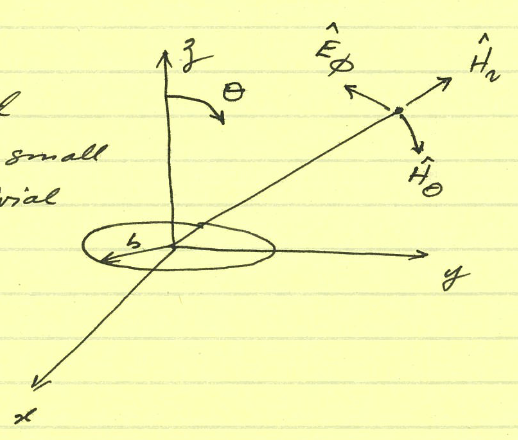
\includegraphics[scale=0.8]{Course Notes/images/7.1.png}
  \caption{Small loop antenna centered around the origin on the $xy$ plane}
\end{figure}

Note that the units of the magnetic dipole moment are amperes meter-squared $[A m^2]$ 

Finding the field of the electrically small "dipole" is very difficult and skipped here. 

We have the following equations:

\begin{center}
    $\Vec{E_N} = \Vec{E_\theta} = \hat{H_i} = 0$ \\
    \hspace{0.1} \\
    $\Vec{E_\phi} = -j \frac{\omega \mu_0 \hat{m} \beta_0^2}{4 \pi} \sin(\theta) (\frac{j}{\beta_0 r} + \frac{1}{\beta_0^2 r^2})e^{-j \beta_0 r}$ \\
    \hspace{0.1} \\
    $\Vec{H_r} = j 2 \frac{\omega \mu_0 \hat{m} \beta_0^2}{4 \pi \eta_0} \cos(\theta) (\frac{1}{\beta_0^2 r^2} - \frac{j}{\beta_0^3 r^3})e^{-j \beta_0 r}$ \\
    \hspace{0.1} \\
    $\Vec{H_\theta} = j \frac{\omega \mu_0 \hat{m} \beta_0^2}{4 \pi \eta_0} \sin(\theta) (\frac{j}{\beta_0 r} + \frac{1}{\beta_0^2 r^2} - \frac{j}{\beta_0^3 r^3})e^{-j \beta_0 r}$ \\\\
\end{center}

The far field of the magnetic dipole is characterized by the $\frac{1}{r}$-dependent terms. This leverages the fact that as $r \to \infty$, terms that are inversely proportional to $r$ converge to zero. This gives us:

\begin{center}
    $\Vec{E}_{FF} = \frac{\omega \mu_0 \hat{m} \beta_0}{4 \pi} \sin(\theta) (\frac{e^{-j \beta_0 r}}{ r})\hat{a}_\theta$ \\
    \hspace{0.1} \\
    $\Vec{H}_{FF} = -\frac{\omega \mu_0 \hat{m} \beta_0}{4 \pi \eta_0} \sin(\theta) (\frac{e^{-j \beta_0 r}}{ r})\hat{a}_\theta$ \\
    
\end{center}

Note that the $\frac{1}{r}$-dependent terms have a $\beta$ term in the denominator as well. This results in the squared $\beta$ in the numerator of the first term being reduced to a first order term.

We can contrast this with the far field of the electrically-small electric dipole and we find there are strong similarities. For the electrically small electric dipole of length $l$:

\begin{center}
    
    $H_N = H_\theta = E_\phi = 0$ \\
    \hspace{0.1} \\
    $H_\theta = j \frac{k I_0 l \sin(\theta)}{4\pi} (1 + \frac{1}{\gamma k r}) e^{-j k r}$ \\
    \hspace{0.1} \\
    $E_N = \eta \frac{ I_0 l \cos(\theta)}{2 \pi r^2} (1 + \frac{1}{\gamma k r}) e^{-j k r}$ \\
    \hspace{0.1} \\ 
    $E_\theta = j \eta \frac{k I_0 l \sin(\theta)}{4\pi r} (1 + \frac{1}{\gamma k r} - \frac{1}{(kr)^2}) e^{-j k r} $ \\

\end{center}

Now, recall Maxwell's Equations in free space:

\begin{itemize}
    \item \textbf{Faraday Law}: $\triangledown \times \Vec{E} = -j\omega \mu \hat{H}$
    \item \textbf{Ampere Law}: $\triangledown \times \Vec{H} = j \omega \epsilon \Vec{E} + \Vec{J}$
    \begin{itemize}
        \item $\Vec{J}$ is an independent source
    \end{itemize}
\end{itemize}

Suppose that we \textit{imagine} a magnetic current, $\Vec{M}$, which would fit into Maxwell's Equations such that:

\begin{itemize}
    \item \textbf{Faraday Law}: $\triangledown \times \Vec{E} = -j\omega \mu \hat{H} - \Vec{M}$
    \item \textbf{Ampere Law}: $\triangledown \times \Vec{H} = j \omega \epsilon \Vec{E}$

\end{itemize}

Notice the similarities between the two systems shown above.  This suggests that a magnetic dipole of magnetic moment $I_m l$ (with $I_m$ is the magnitude of the magnetic current, and $l$ is the length), is \textit{equivalent} to a small electric loop of radius $a$ and constant electric current $I_0$, provided that:

\begin{center}
    $I_m l = js\omega \mu I_0$, where $s = \pi a^2$
\end{center}

Some observations:

\begin{itemize}
    \item The far field radiation contains two field $\Vec{E}, \Vec{H}$ components int he plane perpindicular to the radial vector (as we expect). The near field story, hwoever, is more interesting.
    \item Very close to the loop, the higher order $\frac{1}{kr}$-dependent terms dominate (the opposite of what happens in the far field!)
    \item As $kr << 1$: 
\begin{center}
    $\Vec{H_r} \to j k r^2 I_0 \cos(\theta) \frac{1}{2 j k r^3} e^{-jkr} $ \\
    \hspace{0.1} \\
    $\Vec{H_\theta} \to -(k a)^2 I_0 \sin(\theta) \frac{1}{4 k^2 r^3} e^{-jkr} $ \\
    \hspace{0.1} \\
    $\Vec{E_\theta} \to \eta (k a)^2 I_0 \sin(\theta) \frac{1}{4 j k r^2} e^{-jkr} $ \\

\end{center}

    \item Interestingly, the $H$ field is appearably higher than the $E$ field in the near field to the loop.
    
    \begin{itemize}
        \item This observation is important as it suggests that it could make a huge difference where the loop is used as a probe to test material morphology or composition
        \item For example, if one is testing/probing magnetic material, a small loop probe is more effective than a dipole/electric probe.
    \end{itemize}

\end{itemize}

\section{In-Lecture Notes}

We have to be careful where the small loop is valid. If the circumference is a wavelength or more, we cannot use the calculations shown in the lecture notes. 

If we have an electrically small loop antenna, how can we model it? When we are modelling something, we are trying to convert it to a circuit so that we can perform circuit analysis. Therefore, we can use a resistor, capacitor and inductor to model our electrically small loop antenna.

\begin{itemize}
    \item \textbf{Inductance}, $L$ comes from the fact that we have a loop, which causes a magnetic flux to form via the flow of current that gives rise to the magnetic field.
    \item \textbf{Capacitance} $C$ comes from the inherent capacitance that forms between our loop and ground
    \item \textbf{Resistance} $R$ comes from the ohmic losses of our circuit.
\end{itemize}

This gives us an RLC circuit model, with a capacitance in parralel with a resistor and inductor.

Note that we can only do this if the loop is electrically small. If the loop is not electrically small, the model depends strongly on the frequency so we would need to distribute our model across multiple RLC models acting at different frequencies.

Both $C$ and $L$ should instead be written as $C(\omega)$ and $L(\omega)$, since they are functions of frequency.

As $R \to 0$, the impedance goes to just $R$, since the inductor becomes a short and the capacitor becomes an open.


\end{document}